In questa esperienza si vuole controllare un display a 7 segmenti mediante un programma Arduino. Sono stati utilizzati i seguenti componenti:
\begin{itemize}
    \item Resistenze $R_1=\dots=R_7$ da determinare, 0.25 W.
    \item Display a 7 segmenti,  codice \textit{SC05-11GWA}, Kingbright 
    \item Scheda Arduino DUE
\end{itemize}
Il circuito riportato in Figura \ref{fig:Circuit3} è alimentato mediante porta USB del PC, la quale eroga circa $(\sim 5 V)$
\begin{figure}[H]
    \centering
    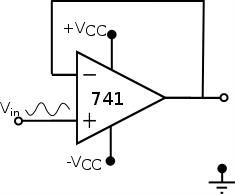
\includegraphics[width=0.5\linewidth]{images/Circuit3.png}
    \caption{Schema circuito (solo alcuni dei LED) e layout del display}
    \label{fig:Circuit3}
\end{figure}
I vari LED del display a 7 segmenti sono collegati ai pin digitali \textbf{12\dots6}
\subsection{Dimensionamento circuito - prelab}
Si è calcolato il valore delle resistenze $R_i$ che permette di ottenere una corrente di 3 mA su ciascun LED. Sapendo che i LED del display hanno tensione operativa pari a $V_{ON}=...\text{ V}$
\begin{equation*}
    R_1=\dots=R_7=1\text{ k}\Omega, 0.25\text{ W}
\end{equation*}
\clearpage
\subsection{Codice}
Si è scritto un programma che visualizza sul display a 7 segmenti un valore numerico (da 0 a 9) proporzionale al tempo trascorso dall’inizio del programma (in secondi); il contatore viene azzerato quando sono trascorsi 10 s. Il codice è riportato in seguito.
\begin{lstlisting}[frame=single, language=Arduino]
const int segPin[7] = {12,11,10,9,8,7,6};   // Pins for the 7 segments

const bool numbers[10][7] = {
    {1,1,1,0,1,1,1},    // 0
    {1,0,0,0,1,0,0},    // 1
    {1,1,0,1,0,1,1},    // 2
    {1,1,0,1,1,1,0},    // 3
    {1,0,1,1,1,0,0},    // 4
    {0,1,1,1,1,1,0},    // 5
    {0,1,1,1,1,1,1},    // 6
    {1,1,0,0,1,0,0},    // 7
    {1,1,1,1,1,1,1},    // 8
    {1,1,1,1,1,1,0}     // 9
};

void setup(){
    for(int i=0; i<7; i++){
        pinMode(segPin[i], OUTPUT); // puts all digital pin as OUTPUT
    }
}

void loop(){
    for(int num = 0; num < 10; num++){
        for(int i=0; i<7; i++){
            digitalWrite(segPin[i], numbers[num][i]);
        }
        delay(1000);
    }
}
\end{lstlisting}
Abbiamo definito nel codice un array bidimensionale di tipo \texttt{bool} che contiene per ognuna delle 10 cifre binarie la corrispondente sequenza di 7 valori logici che permette di visualizzare la cifra stessa. Nel programma sia va a selezionare dalla matrice il numero e il segmento per sapere se tale segmento va acceso o meno.\\\\
E' possibile apprezzare il funzionamento del circuito dal video al \href{https://mediaspace.unipd.it/media/Esperimento+3/1_pnzjn046}{seguente link}